\chapter{Localized Questions in Medical Visual Question Answering}
\label{chapter:locvqa}
% MICCAI 2023 paper about localized questions

The task of \gls{vqa} has seen a relatively rapid development since it was first introduced back in 2015. With a few exceptions, \gls{vqa} models have been applied to datasets with questions that refer to the entire image. This, however, can limit the interpretability of the model's predictions, as the model can benefit from biases in the data to produce the correct answer while disregarding the parts of the image that contain key information to answer the question. Furthermore, localized questions allow the comparison and quantification of agreement between questions about images and questions about regions. In this work, we present an attention-based method for medical \gls{vqa} that enables the posing of questions about specific user-defined regions of an image while considering the context required to answer them. We benchmark our approach across multiple datasets and against different baselines, showing its effectiveness. 

\textbf{Author Contribution} The contributing authors to this work are Pablo Márquez-Neila and Raphael Sznitman. My contributions to this chapter include the creation of the datasets, the development of the methodology, the conception and realization of the experiments, data analysis and interpretation, and visualization as well as the writing of the manuscript.

\textbf{Publication}  This work is published in the Proceedings of the MICCAI 2023 conference \cite{tascon2023localized}.

\newpage

% Paper contents
\section{Background and Previous Work}
\label{sec:locvqa_locatt_background}

\gls{vqa} models are neural networks that answer natural language questions about an image~\cite{antol2015vqa,goyal2017making,hudson2019gqa,tan2019lxmert}. The capability of \gls{vqa} models to interpret natural language questions is of great appeal, as the range of possible questions that can be asked is vast and can differ from those used to train the models. This has led to many proposed \gls{vqa} models for medical applications in recent years~\cite{ImageCLEFVQA_Med2018,liu2019effective,liao2020aiml,vu2020question,zhan2020medical,gong2021cross,yu2023question}. These models can enable clinicians to probe the model with nuanced questions, thus helping to build confidence in its predictions.

Recent work on \gls{medvqa} has primarily focused on building more effective model architectures~\cite{gong2021cross,ren2020cgmvqa,vu2020question} or developing strategies to overcome limitations in \gls{medvqa} datasets~\cite{Nguyen19,liu2021slake,pelka2018radiology,do2021multiple,vu2020question}. Another emerging trend is to enhance \gls{vqa} performance by addressing the consistency of answers produced~\cite{tascon2022consistency}, particularly when considering entailment questions (\ie, the answer to ``Is the image that of a healthy subject?" should be consistent with the answer to ``Is there a fracture in the tibia?"). Despite these recent advances, however, most \gls{vqa} models are restricted to questions that consider the entire image at a time. Specifically, \gls{vqa} typically uses questions that address content within an image without specifying where this content may or may not be in the image. Yet the ability to ask specific questions about regions or locations of the image would be highly beneficial to any user as it would allow fine-grained questions and model probing. For instance, Fig.~\ref{fig:examples_data} illustrates examples of such \emph{localized questions} that combine content and spatial specifications. In the medical field, posing localized questions can significantly enhance the diagnostic process by providing second opinions to medical experts about suspicious regions. Additionally, this approach can improve trustworthiness by assessing the consistency between answers to both global and localized questions.

To this day, few works have addressed the ability to include location information in \gls{vqa} models. In~\cite{mani2020point}, localization information is posed in questions by constraining the spatial extent to a point within bounding boxes yielded by an object detector. The model then focuses its attention on objects close to this point. However, the method was developed for natural images and relies heavily on the object detector to limit the attention extent, making it difficult to scale in medical imaging applications. Alternatively, the approach from~\cite{vu2020question} answers questions about a pre-defined coarse grid of regions by directly including region information into the question (\eg, ``Is grasper in (0,0) to~(32,32)?"). This method relies on the ability of the model to learn a spatial mapping of the image and limits the regions to be on a fixed grid. Localized questions were also considered in~\cite{tascon2022consistency}, but the region of interest was cropped before being presented to the model, assuming that the surrounding context is irrelevant for answering this type of question.
\begin{figure}[!t]
\begin{center}
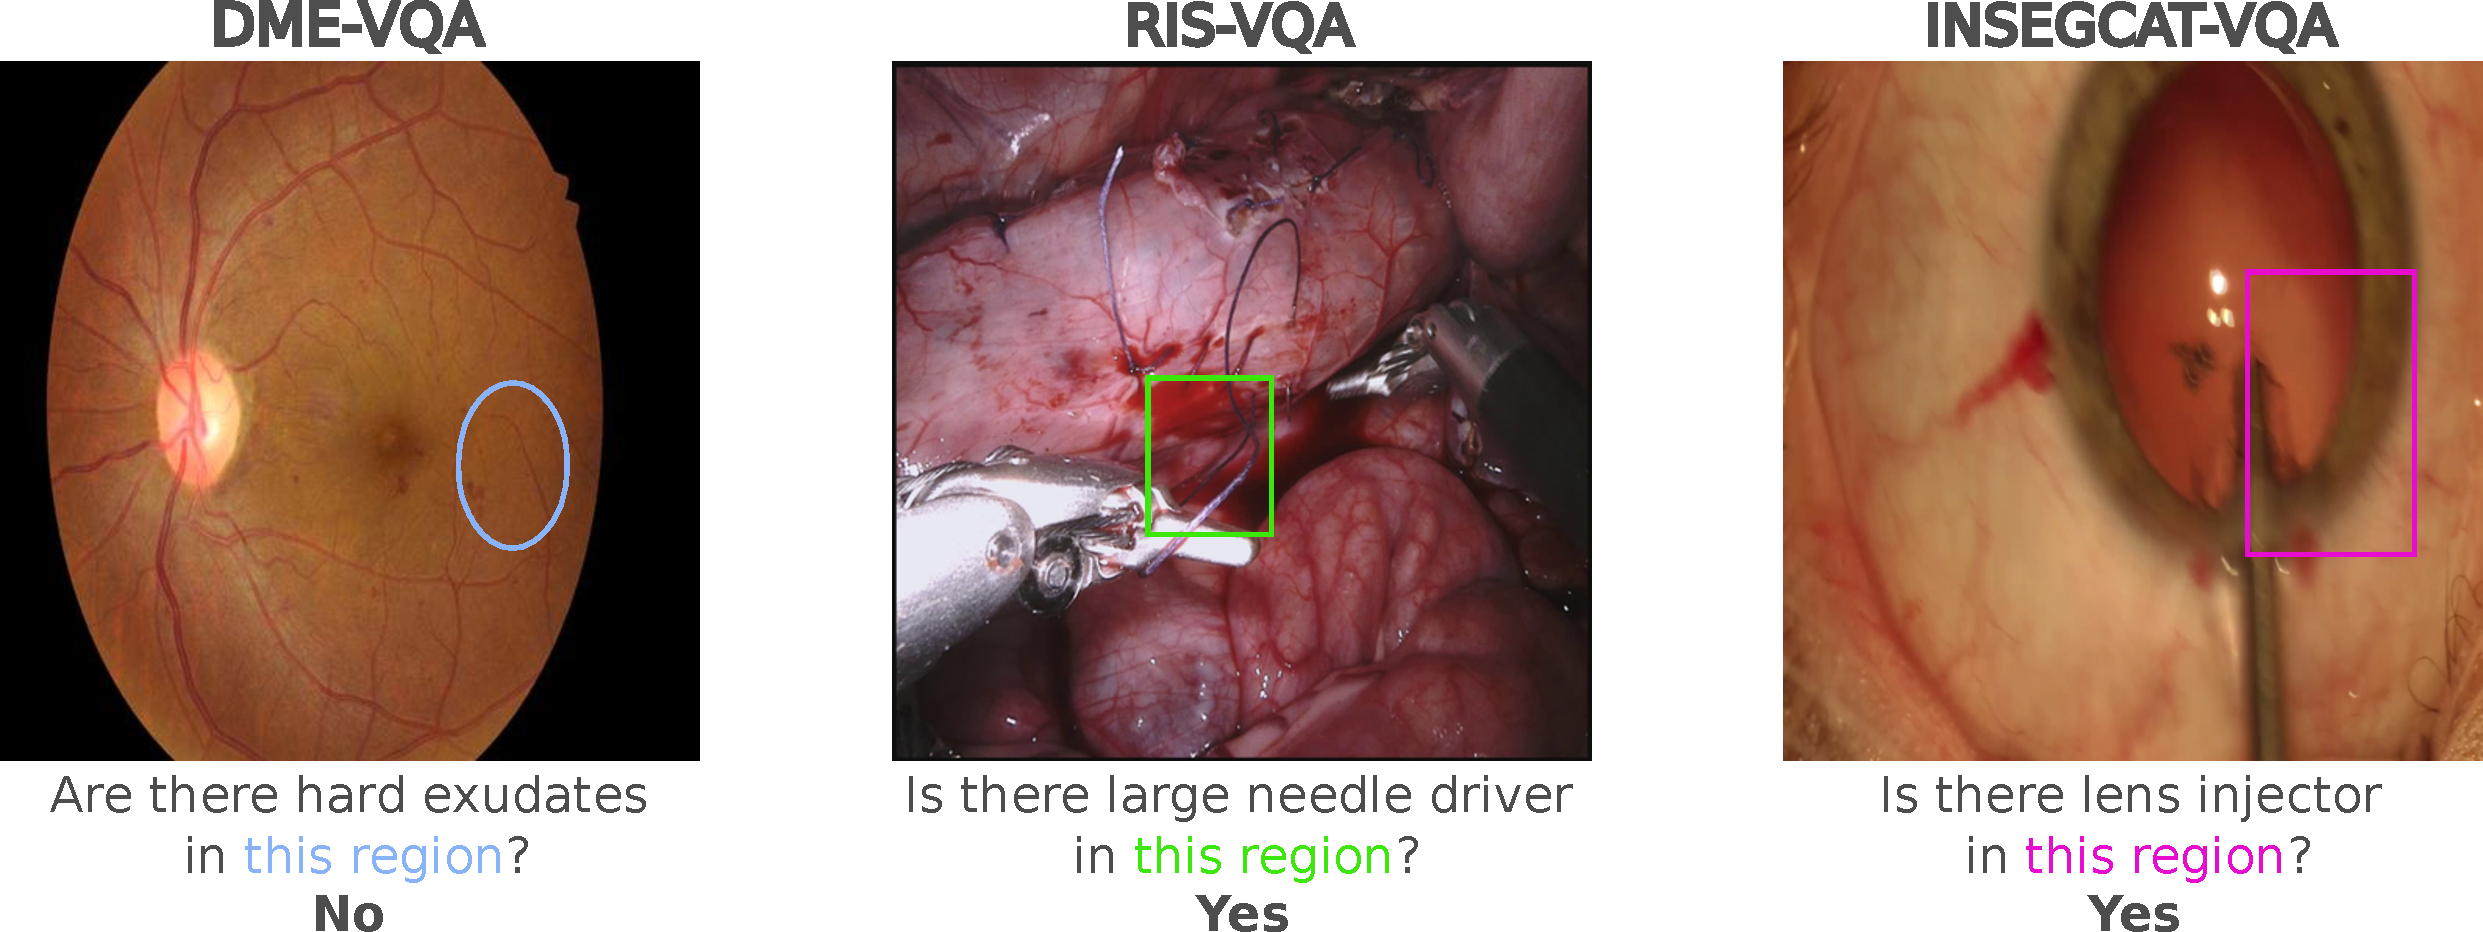
\includegraphics[width=0.9\textwidth]{Figures/Part1_LocVQA/01_locatt/examples_data.pdf}
\caption{Examples of localized questions. In some cases (RIS-VQA and INSEGCAT-VQA), the object mentioned in the question is only partially present in the region. We hypothesize that context can play an important role in answering such questions.}
\label{fig:examples_data}
\end{center}
\end{figure}

To overcome these limitations, we propose a novel \gls{vqa} architecture that alleviates the mentioned issues. At its core, we hypothesize that by allowing the \gls{vqa} model to access the entire images and properly encoding the region of interest, this model can be more effective at answering questions about regions. To achieve this, we propose using a multi-glimpse attention mechanism~\cite{ben2017mutan,vu2020question,tascon2022consistency} restricting its focus range to the region in question, but only after the model has considered the entire image. By doing so, we preserve contextual information about the question and its region. We evaluate the effectiveness of our approach by conducting extensive experiments on three datasets and comparing our method to state-of-the-art baselines. Our results demonstrate performance improvements across all datasets. 
\section{Method}
\label{sec:locvqa_locatt_method}

Our method extends a \gls{vqa} model to answer localized questions. We define a \emph{localized question} for an image~$\x$ as a tuple~$(\q, \m)$, where $\q$~is a question, and $\m$~is a binary mask of the same size as~$\x$ that identifies the region to which the question pertains. Our \gls{vqa} model, parameterized by $\bm{\theta}$ and depicted in Fig.~\ref{fig:method_locvqa}, accepts an image and a localized question as input and produces a probability distribution over a finite set~$\mathcal{A}$ of possible answers. The final answer~$\hat{a}$ of the model is the element with the highest probability,
\begin{equation}
    \hat{a} = \argmax_{a\in\mathcal{A}} p(a\mid \q, \x, \m; \bm{\theta}).
\end{equation}
The model proceeds in three stages to produce its prediction: input embedding, localized attention, and final classification.

\subsection{Input Embedding} The question~$\q$ is first processed by an \gls{lstm}~\cite{hochreiter1997long} to produce an embedding~$\hat{\q}\in\real^Q$. Similarly, the image~$\x$ is processed by a ResNet-152~\cite{he2016deep} to produce the feature map~$\hat{\x}\in\real^{C\times{}H\times{}W}$.

\subsection{Localized Attention} An attention mechanism uses the embedding to determine relevant parts of the image to answer the corresponding question. Unlike previous attention methods, we include the region information that the mask defines. Our \emph{localized attention} module (Fig.~\ref{fig:method_locvqa} right) uses both descriptors and the mask to produce multiple weighted versions of the image feature map,~$\hat{\x}'=\att(\hat{\q}, \hat{\x}, \m)$. To do so, the module first computes an attention map~$\g\in\real^{G\times{}H\times{}W}$ with $G$~glimpses by applying unmasked attention~\cite{kim2016hadamard,vu2020question} to the image feature map and the text descriptor. The value of the attention map at location~$(h, w)$ is computed as,
\begin{equation}
    \g_{:hw} = \textrm{softmax}\left(\W^{(g)}\cdot\textrm{ReLU}\left(\W^{(x)}\hat{\x}_{:hw} \odot \W^{(q)}\hat{\q}\right)\right),
\end{equation}
where the index ${:}hw$ indicates the feature vector at location~$(h, w)$, $\W^{(x)}\in\real^{C'\times C}$, $\W^{(q)}\in\real^{C'\times Q}$, and $\W^{(g)}\in\real^{G\times C'}$ are learnable parameters of linear transformations, and $\odot$~is the element-wise product. In practice, the transformations $\W^{(x)}$ and $\W^{(g)}$ are implemented with $1\times{}1$~convolutions and all linear transformations include a dropout layer applied to its input. The image feature maps~$\hat{\x}$ are then weighted with the attention map and masked with~$\m$ as,
\begin{equation}
    \hat{\x}'_{cghw} = \g_{ghw} \cdot \hat{\x}_{chw} \cdot \left(\m\downarrow_{H\times{}W}\right)_{hw},
\end{equation}
where $c$ and~$g$ are the indexes over feature channels and glimpses, respectively, $(h, w)$~is the index over the spatial dimensions, and $\m\downarrow_{H\times{}W}$~denotes a binary downsampled version of~$\m$ with the spatial size of~$\hat{\x}$. This design allows the localized attention module to compute the attention maps using the full information available in the image, thereby incorporating context into them before being masked to constrain the answer to the specified region.

\subsection{Classification} The question descriptor~$\hat{\q}$ and the weighted feature maps~$\hat{\x}'$ from the localized attention are vectorized and concatenated into a single vector of size~$C\cdot{}G + Q$ and then processed by a multi-layer perceptron classifier to produce the final probabilities.

\subsection{Training} The training procedure minimizes the standard cross-entropy loss over the training set updating the parameters of the \gls{lstm} encoder, localized attention module, and the final classifier. The training set consists of triplets of images, localized questions, and the corresponding ground-truth answers. As in~\cite{antol2015vqa}, the ResNet weights are fixed with pre-trained values, and the \gls{lstm} weights are updated during training.

\begin{figure}[!t]
\begin{center}
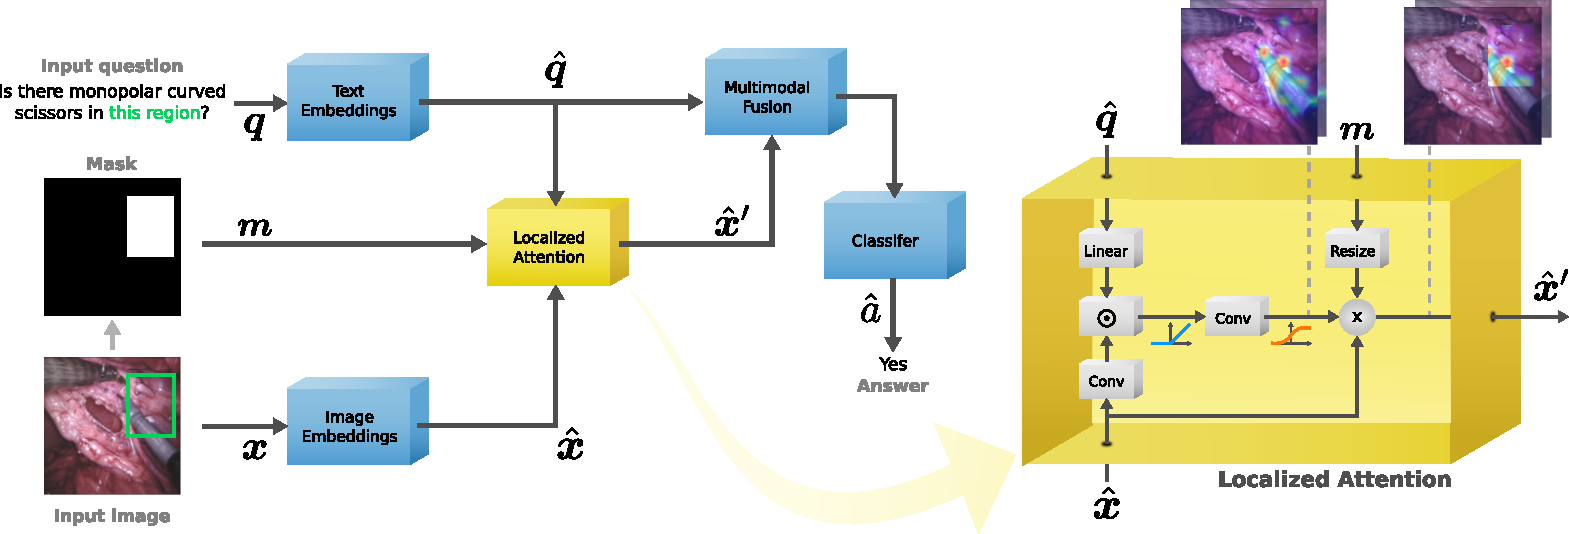
\includegraphics[width=0.99\textwidth]{Figures/Part1_LocVQA/01_locatt/method_new.pdf}
\caption{\textbf{Left:} Proposed VQA architecture for localized questions. The Localized Attention module allows the region information to be integrated into the VQA while considering the context necessary to answer the question. \textbf{Right:} Localized Attention module.  
}
\label{fig:method_locvqa}
\end{center}
\end{figure}
\section{Experiments and Results}
\label{sec:locvqa_locatt_experiments_and_results}

We compare our model to several baselines across three datasets and report quantitative and qualitative results. Additional results are available in Appendix~\ref{appendix:locvqa}. 

\subsection{Datasets}
\label{subsec:locvqa_datasets}
We evaluate our method on three datasets containing questions about regions which we detail here. The first dataset consists of an existing retinal fundus \gls{vqa} dataset with questions about the image's regions and the entire image. The second and third datasets are generated from public segmentation datasets but  use the method described in~\cite{vu2020question} to generate a \gls{vqa} version with region questions. %Fig.~\ref{fig:examples_data} illustrates examples of question-answer pairs in these datasets which we describe in more detail here:
\begin{description}
    \item[\gls{dme}-VQA~\cite{tascon2022consistency}:] 679~fundus images containing questions about entire images (\eg,~``what is the \gls{dme} risk grade?") and about randomly generated circular regions (\eg,~``are there hard exudates in this region?"). The dataset comprises 9'779~question-answer~(QA) pairs for training, 2'380~for validation, and 1'311 for testing.
    \item[RIS-VQA:] Images from the 2017~Robotic Instrument Segmentation dataset~\cite{allan20192017}. We automatically generated binary questions with the structure ``is there [instrument] in this region?" and corresponding masks as rectangular regions with random locations and sizes. Based on the ground-truth label maps, the binary answers were labeled ``yes'' if the region contained at least one pixel of the corresponding instrument and ``no'' otherwise. The questions were balanced to maintain the same amount of ``yes'' and ``no'' answers. 15'580~QA pairs from 1'423 images were used for training, 3'930 from 355 images for validation, and 13'052 from 1'200 images for testing.
    %Though not reported in the paper, we also experimented with other thresholds to define positive answers. For example, making the threshold dependent on region area (1\%), or by using 10 px as threshold. In both cases, we observed significantly better performance in our method. For example, using the mentioned thresholds on the RIS-VQA dataset, our method has an AUC 0.04 higher than the baseline Crop Region, which is very similar to the difference reported in the paper (0.05). We considered 1 px the least arbitrary threshold and reported results for it
    \item[INSEGCAT-VQA:] Frames of cataract surgery videos from the InSegCat~2 dataset~\cite{fox2020insegcat}. We followed the same procedure as in RIS-VQA to generate balanced binary questions with masks and answers.
    The dataset consists of 29'380~QA pairs from 3'519 images for training, 5'306 from 536 images for validation, and 4'322 from 592 images for testing. % also in this case with 50\% Yes and 50\% No questions. 
\end{description}
Fig.~\ref{fig:object_distribution} shows the distribution of questions in the three datasets.

\begin{figure}[t]
\begin{center}
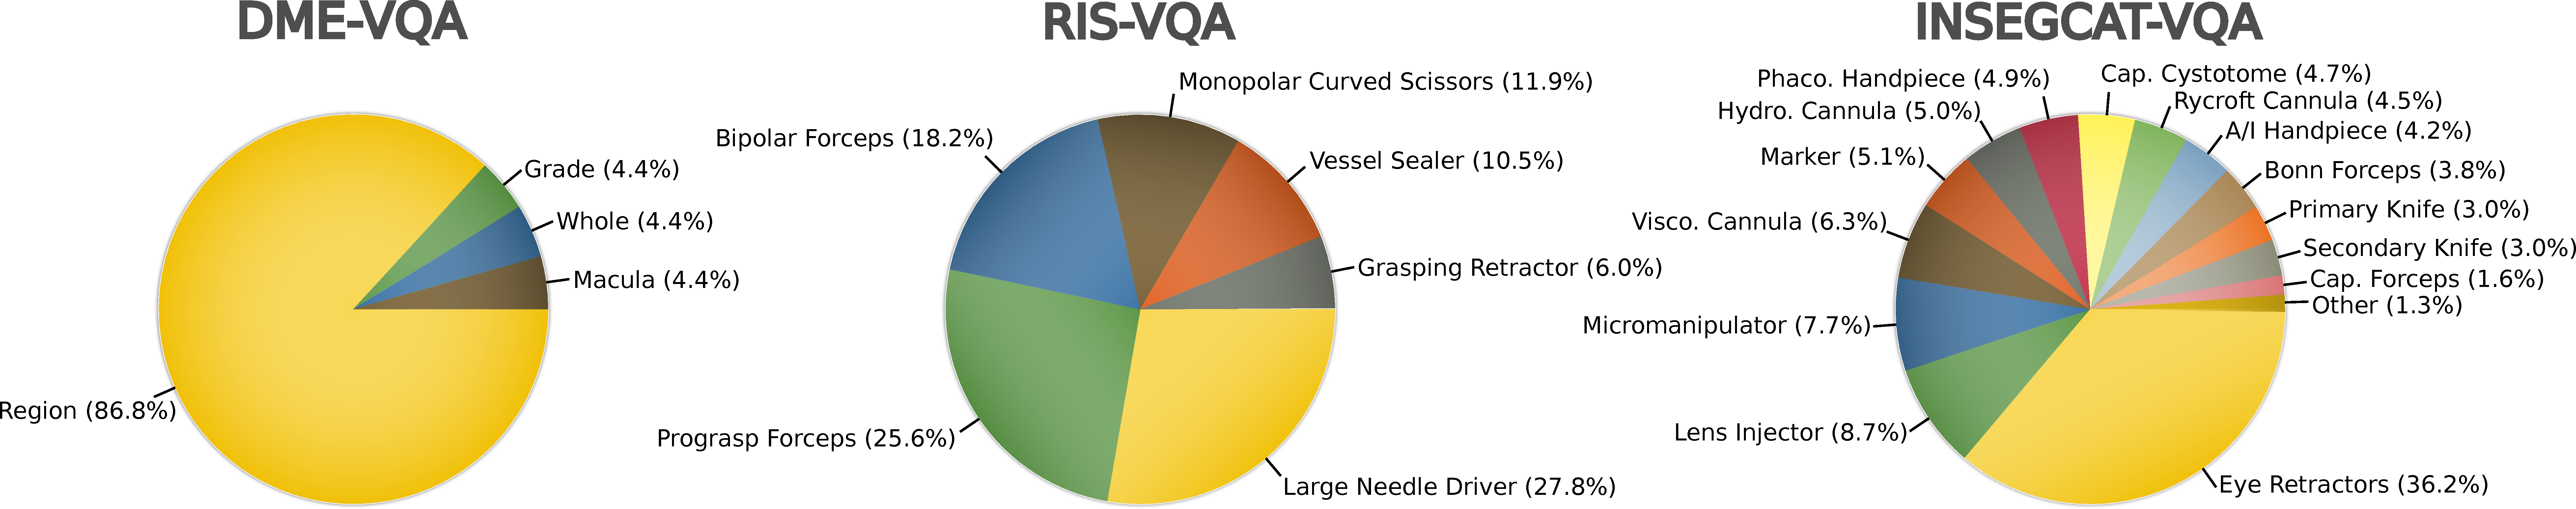
\includegraphics[width=\textwidth]{Figures/Part1_LocVQA/01_locatt/pie_charts_data.pdf}
\caption{Distribution by question type (DME-VQA) and by question object (RIS-VQA and INSEGCAT-VQA).}
\label{fig:object_distribution}
\end{center}
\end{figure}

\subsection{Baselines and Metrics}
We compare our method to four different baselines, as shown in Fig.~\ref{fig:baselines}:
\begin{description}
    \item[No mask:] no information is provided about the region in the question.
    \item[Region in text~\cite{vu2020question}:] region information is included as text in the question.
    \item[Crop region~\cite{tascon2022consistency}:] image is masked to show only the queried region, with the area outside the region set to zero.
    \item[Draw region:] region is indicated by drawing its boundary on the input image with a distinctive color.
\end{description}
We evaluated the performance of our method using accuracy for the DME-VQA dataset and the area under the \gls{roc} curve and Average Precision (AP) for the RIS-VQA and INSEGCAT-VQA datasets.

\begin{figure}[!t]
\begin{center}
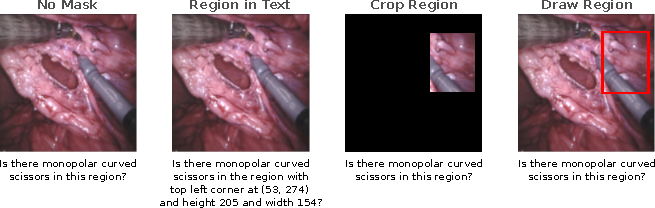
\includegraphics[width=0.98\textwidth]{Figures/Part1_LocVQA/01_locatt/baselines.pdf}
\caption{Illustration of the evaluated baselines for an example image.}
\label{fig:baselines}
\end{center}
\end{figure}

\subsubsection{Implementation Details}

Our \gls{vqa} architecture uses an \gls{lstm}~\cite{hochreiter1997long} with an output dimension~1024 to encode the question and a word embedding size of~300.
% The question length is~12 for normal questions and 21 when the region information is included in the question \PMN{Why do we need to specify this? It sounds strange that we have two exact kinds of questions.}. \STM{Questions with region info are naturally longer, so they require a bigger vector size. It's not essential to mention it.} 
We use the ResNet-152~\cite{he2016deep} with ImageNet weights to encode images of size 448$\times$448, generating feature maps with 2048~channels.
% For multimodal fusion, we use concatenation.
In the localized attention block, the visual and textual features are projected into a 512-dimensional space before being combined by element-wise multiplication. Following \cite{fukui2016multimodal,kim2016hadamard}, the number of glimpses is set to $G=2$ for all experiments.
The classification block is a multi-layer perceptron with a hidden layer of~1024 dimensions. A dropout rate of~0.25 and \gls{relu} activation are used in the localized attention and classifier blocks.

We train our models for 100~epochs using an early stopping condition with patience of 20~epochs. Data augmentation consists of horizontal flips. We use a batch size of 64~samples and the Adam optimizer with a learning rate of $10^{-4}$, which is reduced by a factor of 0.1 when learning stagnates.
% For the DME-VQA dataset, we used weighted cross-entropy, and for the other datasets, we used binary cross-entropy.
Models implemented in PyTorch 1.13.1 and trained on an Nvidia RTX 3090 graphics card\footnote{Our code and data are available at \url{https://github.com/sergiotasconmorales/locvqa}}. 

%%%%%%%%%%%%%%%%%%%%%%%%%%%%%%%
% Results                     %
%%%%%%%%%%%%%%%%%%%%%%%%%%%%%%%

\subsection{Results} 

\label{sec:locvqa_results}


% Table~\ref{tab:locvqa_results_dme} summarizes the results obtained on the DME-VQA dataset for all methods and each type of question. Table~\ref{tab:results_ris_insegcat} shows the RIS-VQA and INSEGCAT-VQA datasets results. Additionally, Table~\ref{tab:results_ris_object} reports the performances for questions pertaining to each type of instrument in the RIS-VQA dataset.  

\begin{table}[!t]
\begin{center}
\begin{tabular}{llp{0.1cm}lp{0.1cm}lp{0.1cm}lp{0.1cm}c}
%
\toprule
\multicolumn{1}{l}{\multirow{2}{*}{Method}} & \multicolumn{9}{c}{Accuracy (\%)}                                                                                                                                               \\ \cmidrule{2-10} 
\multicolumn{1}{c}{} & \multicolumn{1}{c}{Overall}      && \multicolumn{1}{c}{Grade}        && \multicolumn{1}{c}{Whole}        && \multicolumn{1}{c}{Macula}       && \multicolumn{1}{c}{Region} \\ \midrule 
No Mask & \multicolumn{1}{c}{61.1 $\pm$ 0.4} && \multicolumn{1}{c}{80.0 $\pm$ 3.7} && \multicolumn{1}{c}{85.7 $\pm$ 1.2} && \multicolumn{1}{c}{\textbf{84.3 $\pm$ 0.5}} && 57.6 $\pm$ 0.4                \\ 
Region in Text~\cite{vu2020question} & \multicolumn{1}{c}{ 60.0 $\pm$ 1.5} && \multicolumn{1}{c}{57.9 $\pm$ 12.5 } && \multicolumn{1}{c}{85.1 $\pm$ 1.9 } && \multicolumn{1}{c}{ 83.2 $\pm$ 2.4} &&     57.7 $\pm$ 1.0        \\ 
Crop Region~\cite{tascon2022consistency}  & \multicolumn{1}{c}{81.4 $\pm$ 0.3} && \multicolumn{1}{c}{78.7 $\pm$ 1.3} && \multicolumn{1}{c}{81.3 $\pm$ 1.7} && \multicolumn{1}{c}{82.3 $\pm$ 1.4} && 81.5 $\pm$ 0.3               \\
Draw Region  & \multicolumn{1}{c}{ 83.0 $\pm$ 1.0} && \multicolumn{1}{c}{79.6 $\pm$ 2.5 } && \multicolumn{1}{c}{77.0 $\pm$ 4.8 } && \multicolumn{1}{c}{84.0 $\pm$ 1.9 } &&   83.5 $\pm$ 1.0               \\ 
\ours                                          & \multicolumn{1}{c}{\textbf{84.2 $\pm$ 0.6}} && \multicolumn{1}{c}{\textbf{82.8 $\pm$ 0.4}} && \multicolumn{1}{c}{\textbf{87.0 $\pm$ 1.2}} && \multicolumn{1}{c}{83.0 $\pm$ 1.5} && \textbf{84.2 $\pm$ 0.7}                \\ \bottomrule
\end{tabular}
\end{center}
\caption{Average accuracy for different methods on the DME-VQA dataset. The results shown are the average of 5 models trained with different seeds.}
\label{tab:locvqa_results_dme}
\end{table}


\begin{table}[!t]
\begin{center}
\begin{tabular}{lp{0.5cm}lp{0.5cm}cp{0.5cm}c}
\toprule
Dataset                       && Method         && AUC && AP \\ \midrule
\multirow{4}{*}{RIS-VQA}      && No Mask    && 0.500 $\pm$ 0.000    &&  0.500 $\pm$ 0.000  \\ 
                                && Region in Text~\cite{vu2020question} &&  0.677 $\pm$ 0.002 && 0.655 $\pm$ 0.003 \\ 
                              && Crop Region~\cite{tascon2022consistency}    &&  0.842 $\pm$ 0.002 && 0.831 $\pm$ 0.002      \\  
                              && Draw Region && 0.835 $\pm$ 0.003 && 0.829 $\pm$ 0.003 \\ 
                              && \ours           && \textbf{0.885 $\pm$ 0.003} && \textbf{0.885 $\pm$ 0.003}\\ \midrule
\multirow{4}{*}{INSEGCAT-VQA} && No Mask    &&   0.500 $\pm$ 0.000  &&  0.500 $\pm$ 0.000   \\  
                              && Region in Text~\cite{vu2020question} &&  0.801 $\pm$ 0.012 && 0.793 $\pm$ 0.014 \\ 
                              && Crop Region~\cite{tascon2022consistency}    &&  0.901 $\pm$ 0.002   && 0.891 $\pm$ 0.003   \\  
                              && Draw Region && 0.910 $\pm$ 0.003 && 0.907 $\pm$ 0.005\\  
                              && \ours           &&  \textbf{0.914 $\pm$ 0.002}   && \textbf{0.915 $\pm$ 0.002}   \\ \bottomrule
\end{tabular}
\end{center}
\caption{Average test AUC and AP for different methods on the RIS-VQA and INSEGCAT-VQA datasets. The results shown are the average over 5~seeds.}
\label{tab:results_ris_insegcat}
\end{table}

\begin{table}[!t]
\ra{1.2}
\begin{center}
\begin{tabular}{p{0.1cm}p{0.13\linewidth}p{0.3cm}LKLKLK}
\toprule
{} &\multirow{2}{*}{Method}  & \multicolumn{7}{c}{Instrument Type} \\
\cmidrule{3-9} 
&         && Large Needle Driver & Monopolar Curved Scissors & Vessel Sealer & Grasping Retractor & Prograsp Forceps & Bipolar Forceps \\ \midrule
&\makecell[tl]{No\\Mask}    && \makecell[tc]{0.500 \\ $\pm$0}              & \makecell[tc]{0.500 \\ $\pm$0}                     & \makecell[tc]{0.500 \\ $\pm$0}            & \makecell[tc]{0.500 \\$\pm$0}                 & \makecell[tc]{0.500 \\ $\pm$0}              & \makecell[tc]{0.500 \\ $\pm$0}              \\ 
&\makecell[tl]{Region in\\Text~\cite{vu2020question}} &&   \makecell[tc]{0.717\\$\pm$0.003}                  &   \makecell[tc]{0.674\\$\pm$0.001}                        &     \makecell[tc]{0.620\\$\pm$0.011}          &    \makecell[tc]{0.616\\$\pm$0.020}                &    \makecell[tc]{0.647\\$\pm$0.008}              &  \makecell[tc]{0.645\\$\pm$0.003}               \\ 
&\makecell[tl]{Crop\\Region~\cite{tascon2022consistency}}    && \makecell[tc]{0.913 \\$\pm$0.002}               & \makecell[tc]{0.812 \\$\pm$0.003}                     & \makecell[tc]{0.752\\$\pm$0.009}         & \makecell[tc]{0.715\\$\pm$0.015}              & \makecell[tc]{0.773 \\$\pm$0.003}            & \makecell[tc]{0.798 \\$\pm$0.004}           \\ 
&\makecell[tl]{Draw\\Region} &&       \makecell[tc]{0.915\\$\pm$0.003}              &   \makecell[tc]{0.777\\$\pm$0.003}       &   \makecell[tc]{0.783\\$\pm$0.004}      &  \makecell[tc]{0.709\\$\pm$0.012}       &  \makecell[tc]{0.755\\$\pm$0.004}       &     \makecell[tc]{0.805\\$\pm$0.005}            \\ 
&\ours          && \makecell[tc]{\textbf{0.944}\\$\pm$\textbf{0.001}}               & \makecell[tc]{\textbf{0.837} \\$\pm$\textbf{0.005}}                     & \makecell[tc]{\textbf{0.872} \\$\pm$\textbf{0.008}}         & \makecell[tc]{\textbf{0.720} \\$\pm$\textbf{0.031}}              & \makecell[tc]{\textbf{0.834} \\$\pm$\textbf{0.006}}            & \makecell[tc]{\textbf{0.880} \\$\pm$\textbf{0.003}}           
\\ \bottomrule
\end{tabular}
\end{center}
\caption{Average test AUC for different methods on the RIS-VQA dataset as a function of instrument type. Results are averaged over 5 models trained with different seeds. The corresponding table for INSEGCAT-VQA is available in Appendix~\ref{appendix:locvqa}.
}
\label{tab:results_ris_object}
\end{table}

Our method outperformed all considered baselines on the DME-VQA (Table~\ref{tab:locvqa_results_dme}), the RIS-VQA, and the INSEGCAT-VQA datasets (Table~\ref{tab:results_ris_insegcat}), highlighting the importance of contextual information in answering localized questions. Context proved to be particularly critical in distinguishing between objects of similar appearance, such as the bipolar and prograsp forceps in RIS-VQA, where our method led to an 8~percent point performance improvement (Table~\ref{tab:results_ris_object}). In contrast, the importance of context was reduced when dealing with visually distinct objects, resulting in smaller performance gains as observed in the INSEGCAT-VQA dataset. For example, despite not incorporating contextual information, the baseline \emph{crop region} still benefited from correlations between the location of the region and the instrument mentioned in the question (\eg,~the eye retractor typically appears at the top or the bottom of the image), enabling it to achieve competitive performance levels that are less than 2~percent points lower than our method~(Table~\ref{tab:results_ris_insegcat}, bottom).

% Across the different datasets, we see that our approach consistently provides performance improvements. This highlights the importance of context in answering localized questions but also depends on how necessary context is to differentiate between all the objects that can be asked about. For instance, we notice that questions that involve objects with similar aspects (\eg, bipolar and prograsp forceps in RIS-VQA) can benefit more from context. In contrast, when an object is notably different from every other object in the scene (\eg, hard exudates in DME-VQA), the boost in performance is limited. This is observed especially in the INSEGCAT-VQA, in which the visual similarity of the tools is rather low and where the model that does not have access to context appears to benefit from correlations between the region location and the object mentioned in the question (\eg, the eye retractor appears at the top or the bottom of the image).

Similar to our method, the baseline \emph{draw region} incorporates contextual information when answering localized questions. However, we observed that drawing regions on the image can interfere with the computation of guided attention maps, leading to incorrect predictions (Fig.~\ref{fig:examples_att}, column~4). In addition, the lack of masking of the attention maps often led the model to wrongly consider areas beyond the region of interest while answering questions~(Fig.~\ref{fig:examples_att}, column~1). 

When analyzing mistakes made by our model, we observe that they tend to occur when objects or background structures in the image look similar to the object mentioned in the question~(Fig.~\ref{fig:examples_att}, column~3). Similarly, false predictions were observed when only a few pixels of the object mentioned in the question were present in the region.


%the model confuses other objects or tissue with the referred object or when the attention maps do not focus on the actual referred object \PMN{These two reasons say that the model fails when it is confused, which is a bit of a circular reasoning. What are the properties of the images that make the model fail? Do they have something in common?} \STM{They tend to contain tissue that has the shape of tools, for example. Or they contain two very similar tools. Or only a very small portion of the object is in the region. This of course doesn't explain all errors, but that's what I saw in common} \PMN{Also, we are only showing a single failure example, which might be not enough.} \STM{Added one more failure from INSEGCAT and transposed the image to use the space better} (Fig.~\ref{fig:examples_att}, column~3).

% to analyze:
% Importance of context when questions require context + without context model confuses other objects with objects mentioned in the question (first row of examples figure)
% Why our method is better than drawing the regions (drawn regions can interfere in attention maps)
% Errors are still possible while considering context

\begin{figure}[!t]
\begin{center}
\includegraphics[width=\textwidth]{Figures/Part1_LocVQA/01_locatt/examples_att_small2_transposed.pdf}
\caption{Qualitative examples on the RIS-VQA dataset (columns~1-3), INSEGCAT-VQA (columns~4-5), and DME-VQA (last column). Only the strongest baselines were considered in this comparison. The first row shows the image, the region, and the ground truth answer. Other rows show the overlaid attention maps and the answers produced by each model. Wrong answers are shown in red.}
\label{fig:examples_att}
\end{center}
\end{figure}
\section{Conclusion}

In this work, we proposed a novel \gls{vqa} architecture to answer questions about regions. We compare the performance of our approach against several baselines and across three different datasets. By focusing the model's attention on the region after considering the evidence in the full image, we show how our method brings improvements, especially when the complete image context is required to answer the questions. Future works include studying the agreement between answers to questions about concentric regions, as well as the agreement between questions about images and regions.







